\documentclass[class=article, crop=false]{standalone}
\usepackage{tikz}
\usepackage{subcaption}
\usetikzlibrary{calc}

\begin{document}

\begin{subfigure}{0.45\linewidth}
    \centering
    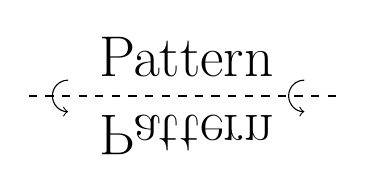
\begin{tikzpicture}
        % Draw the dashed line
        \draw[thick,dashed] (-2,0) -- (2,0);
        % Draw arcs
        \draw[->] (-1.5,0.2) arc (90:270:0.2);
        \draw[->] (1.5,0.2) arc (90:270:0.2);
        % Normal text above the line
        \node at (0,0.5) {\huge Pattern};
        % Mirrored text below the line
            \node[rotate=180] at (0,-0.5) {\reflectbox{\huge Pattern}};
    \end{tikzpicture}
    \caption{Reflections}
    \label{Reflection}
\end{subfigure}
\hfill
\begin{subfigure}{0.45\linewidth}
    \centering
    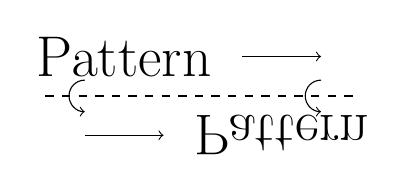
\begin{tikzpicture}
        % Draw the dashed line
        \draw[thick,dashed] (-2,0) -- (2,0);
        % Draw arcs
        \draw[->] (-1.5,0.2) arc (90:270:0.2);
        \draw[->] (1.5,0.2) arc (90:270:0.2);
        % Draw glide
        \draw[->] (0.5,0.5) -- (1.5,0.5);
        \draw[->] (-1.5,-0.5) -- (-0.5,-0.5);
        % Normal text above the line
        \node at (-1,0.5) {\huge Pattern};
        % Mirrored text below the line
            \node[rotate=180] at (1,-0.5) {\reflectbox{\huge Pattern}};
    \end{tikzpicture}
    \caption{Glide Reflection}
    \label{GlideReflection}
\end{subfigure}

\end{document}